\section{Raytracing}

\textit{"schönere" Bilder erzeugen -> Photorealistisch}

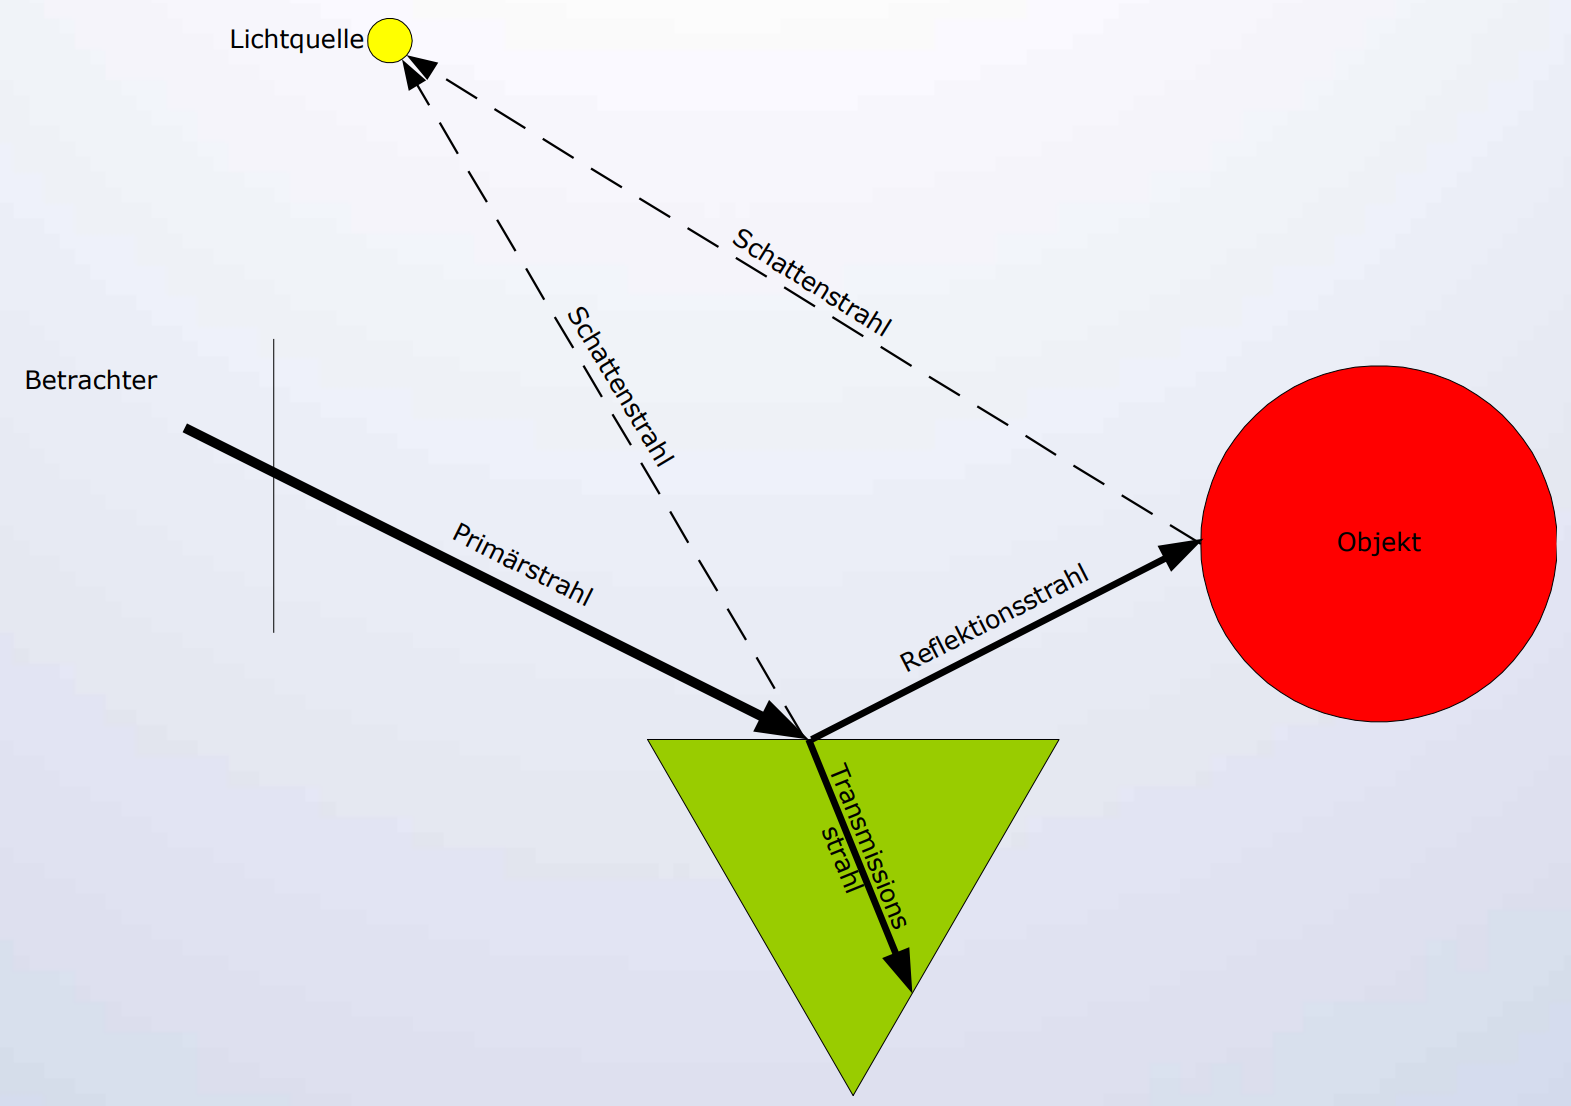
\includegraphics[width=0.4\textwidth]{assets/raytracing-example.png}\\

Strahl durch Pixel -> Schnitt mit nächsten Objekt aus Betrachtung

\textbf{Rekursieves Raytracing} für zusätzliche Effekte \\
\textit{Strahl wird in mehrere Stahlen aufgeteilt;
Spiegelung, Transparenz mit Reflektion, Schatten, (Sampling Umgebungslicht)}\\

\textbf{Beleuchtung} \\
\textit{Wird dadurch errechnet, ob ein aufgetroffener Punkt von einer Lichtquelle beleuchtet ist}\\

\textbf{Ordnung} \\
\textit{definiert die Strahlentiefe / anzahl Reflektionsstrahlen}\\

\textbf{Aliasing} (Adaptives Supersampling) wird viel verwendet \\
\textit{Bild wirkt verpixelt, wenn für jeden Pixel nur einen Strahl verwendet wird}\\

Aufwendige Technik \\
\textit{Um sinnlose Schnitte zu vermeiden ->
Objekte zusammenfassen (Bounding Box) und damit den Schnittpunkt berechnen}\\
\textit{Schnittpunkt mit "Grid" (auf dem Bild) und dann mit Objekten in dieser Zelle}\\

\subsection{Raytracing Ordnung}

\textit{Höhere Ordnung bewirkt mehr Spiegelung und dadurch mehr Detail:}

\begin{enumerate}
    \item Einfach Ordnung, keine Spiegelung
    \item Einfache Rückspiegelung von der Kugel
    \item Ordnung - Boden wird auch gespiegelt
    \item Ordnung noch weitere Spiegelungen und mehr Detail
\end{enumerate}

\subsection{Schnittpunkt Berechnen}

\textit{Die x und y Position mit Nullstellen entsprechen Schnittpunkten}
